% !TEX root = dissertation_BB.tex
%% spellcheck-language en-US

%    #
%   #
%  #  #
%  #####
%     #

\chapter{Real-time, GPU accelerated image processing pipeline}

\graphicspath{{./figures/4_gpu/}}


\section{GPU architecture}
  CUDA \cite{nickolls_scalable_2008}

\section{Live fusion}
  \subsection{MuVi-SPIM}
  \subsection{Bead based registration}



  
\section{B³D image compression}
  \b3d image compression
  high content screening \cite{carpenter_systematic_2004,echeverri_high-throughput_2006,pepperkok_high-throughput_2006}
  light-sheet (Sec. \ref{sec:light-sheet})
  single molecule localization microscopy \cite{betzig_imaging_2006,hess_ultra-high_2006,rust_sub-diffraction-limit_2006}
  data handling is bottleneck \cite{wollman_high_2007,reynaud_guide_2015,perkel_struggle_2016}
  lossy compression not recommended for microscopy  \cite{cromey_digital_2013}
  KLB \cite{amat_efficient_2015}
  jpeg compression so loss is not perceptible \cite{sayood_introduction_2012}
  big data viewer \cite{pietzsch_bigdataviewer:_2015}
  Fiji \cite{schindelin_fiji:_2012}

  FLIC \cite{wang_fast_2012}
  SFALIC \cite{starosolski_simple_2007}
  FELICS \cite{howard_fast_1993}
  Treib terrain editing \cite{treib_interactive_2012}
  Treib turbulence \cite{treib_turbulence_2012}
  square root compression \cite{gowen_square_2003}
  noise and bias in square root compression \cite{bernstein_noise_2010}
  quantization \cite{gray_quantization_1998}
  Anscombe \cite{anscombe_transformation_1948}
  optimal inverse Anscombe \cite{makitalo_optimal_2011,makitalo_closed-form_2011}
  optimal inverse generalized Anscombe \cite{makitalo_optimal_2013}



  \subsection{Data sizes in microscopy}

    \begin{figure}[tpb]
      \centering
      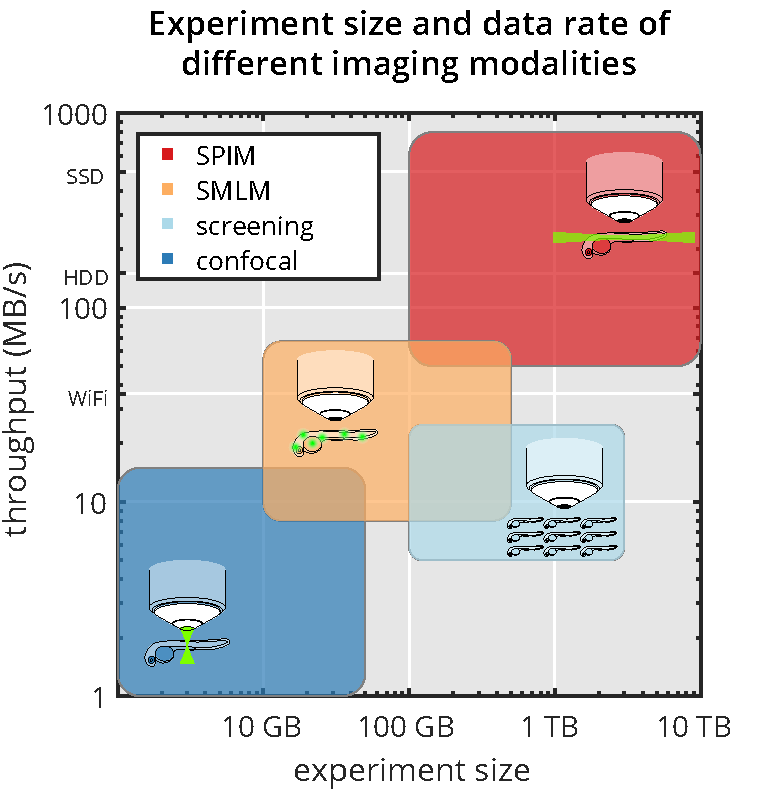
\includegraphics[page=1,width=0.5\textwidth]{comparison_with_pictograms}
      \bcaption[Experiment sizes and data rate of different imaging modalities]{Comparison of single-plane illumination microscopy (SPIM, red rectangle), high-content screening (light blue), single molecule localization microscopy (SMLM, orange) and confocal microscopy (blue) by typical experiment size and data production rate (see also Table \ref{tab:sizes}).}
      \label{fig:sizes}
    \end{figure}


    

  \subsection{Compression algorithm}

    \begin{figure}[tpb]
      \centering
      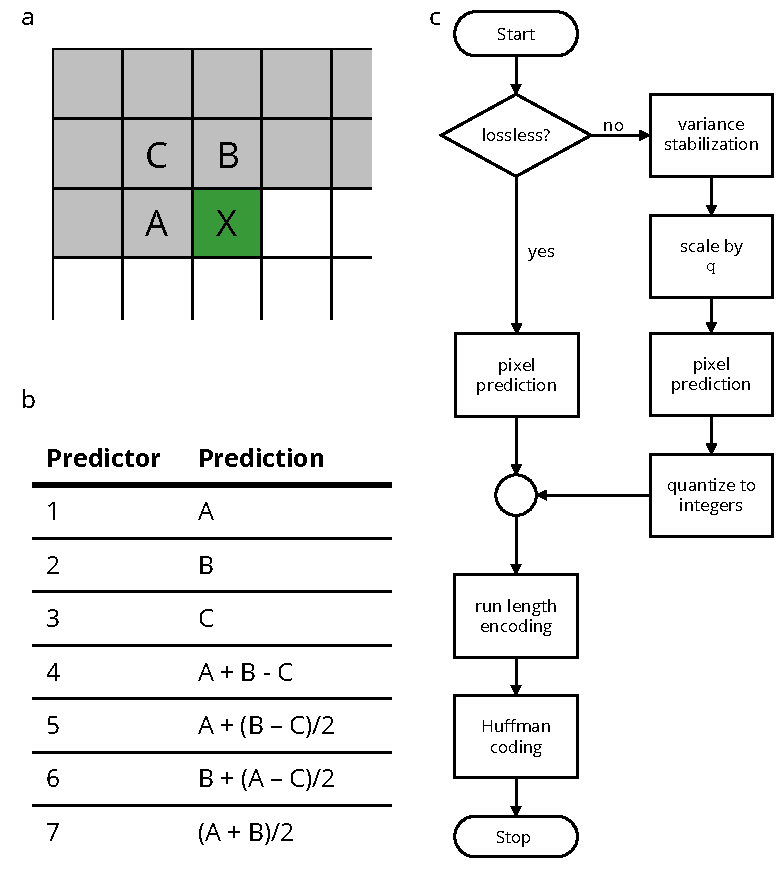
\includegraphics[page=1,width=0.6\textwidth]{SFig1_flow}
      \bcaption[\b3d algorithm schematics]{(\textbf{a}) Prediction context for pixel X, the next sample to be encoded. Three neighboring pixels are considered: left (A), top (B) and top left (C) neighbors. (\textbf{b}) Lossless JPEG predictors for X, based on the context showed in (\textbf{a}). The first three predictors are one-dimensional, while the rest are two-dimensional. Using a two dimensional predictor while increases complexity slightly, also increases the achievable compression ratio. We found that for fluorescence microscopy images predictor 7 performs best, hence its inclusion in the \b3d algorithm. (\textbf{c)} Complete algorithm flowchart depicting the main stages of the compression. First, if the result should be lossless, pixel prediction is performed on the original image values. If within noise level mode is selected, the image noise is stabilized first (see "\textbf{Supplementary Note}"), which is then scaled by the quantization step q. Prediction is performed, and the prediction errors are rounded to the nearest integer. The prediction errors for both lossless and lossy modes are then run-length encoded, and finally Huffman coding is applied to effectively reduce data size. The output of the Huffman coder is saved as the compressed file.}
      \label{fig:algorithm}
    \end{figure}


  \subsection{Lossless compression performance}

    \begin{figure}[tpb]
      \centering
      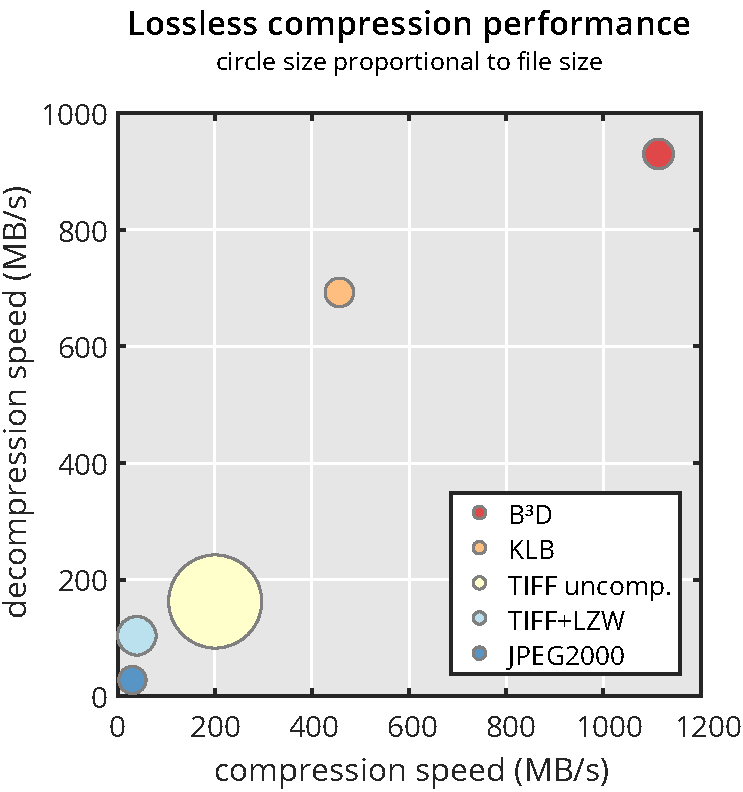
\includegraphics[page=1,height=0.5\textwidth]{bubbles}
      \bcaption[Lossless compression performance]{Performance comparison of our B³D \b3d compression algorithm (red circle) vs. KLB (orange), uncompressed TIFF (light yellow), LZW compressed TIFF (light blue) and JPEG2000 (blue) regarding write speed (horizontal axis), read speed (vertical axis) and file size (circle size). (see also Table \ref{tab:performance}).}
      \label{fig:performance}
    \end{figure}

    


  \subsection{Swapping for WNL}

    \begin{figure}[tpb]
      \centering
      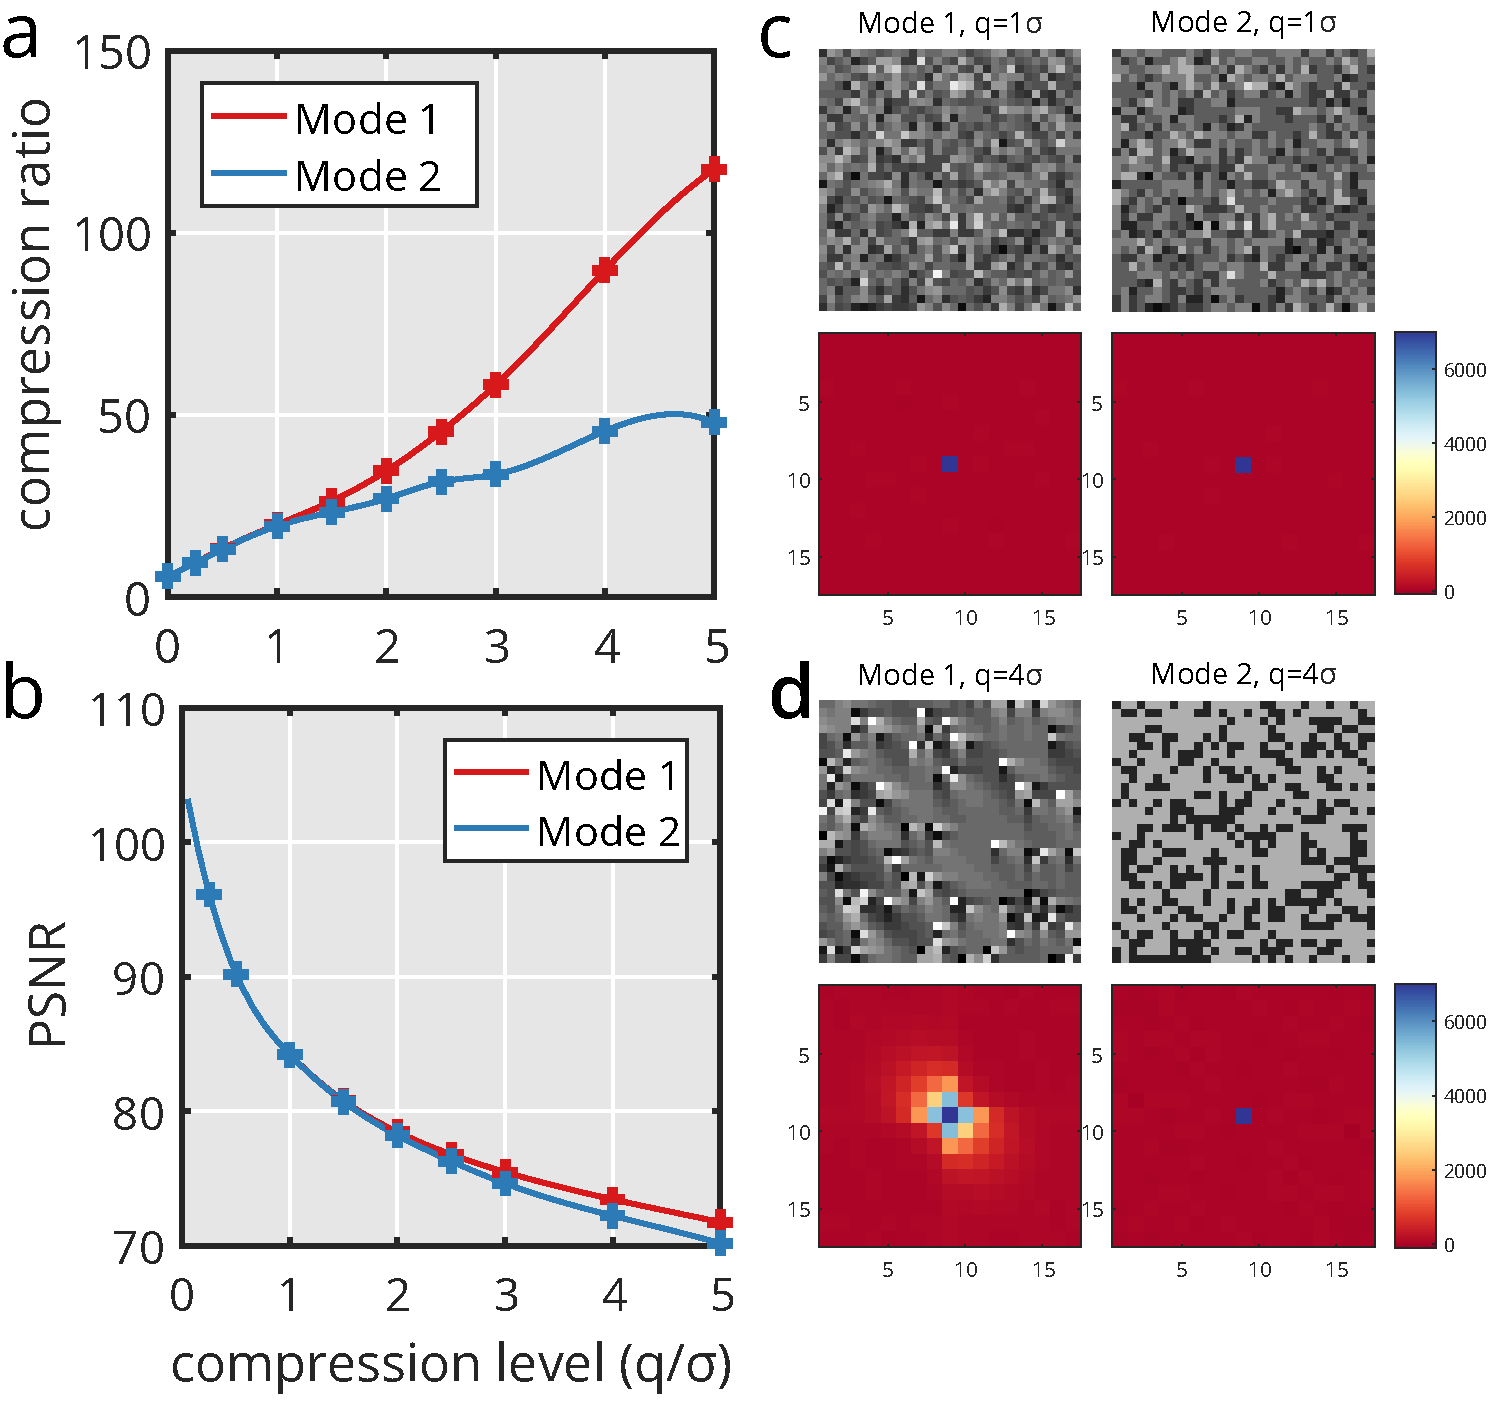
\includegraphics[page=1,width=0.7\textwidth]{swapping}
      \bcaption[Options for noise dependent lossy compression]{Comparing Mode 1 (prediction then quantization) and Mode 2 (quantization then prediction) of noise dependent lossy compression in terms of compression ratio, peak signal to noise ratio (PSNR) and spatial correlations introduced to random noise. (\textbf{a}) Compression ratio as a function of the quantization step for Mode 1 and Mode 2. (\textbf{b}) PSNR as a function of the quantization step for Mode 1 and Mode 2. (\textbf{c, d}) Random noise was compressed at various quantization steps both for Mode 1 and Mode 2. Autocorrelation was calculated for the compressed images to see whether the compression introduces any spatial correlation between the pixels. For q=1$\upsigma$ both modes are free of correlation (\textbf{c}, top: compressed images, bottom: autocorrelation), however, for q=2$\upsigma$ Mode 1 exhibits a correlation pattern (\textbf{d}, top left: compressed image, bottom left: autocorrelation) that is not present in Mode 2 (\textbf{d}, top right compressed image, bottom right: autocorrelation). For more discussion, see "\textbf{Supplementary Note}".}
      \label{fig:swapping}
    \end{figure}

  \subsection{Benchmarking}

    \begin{figure}[tpb]
      \centering
      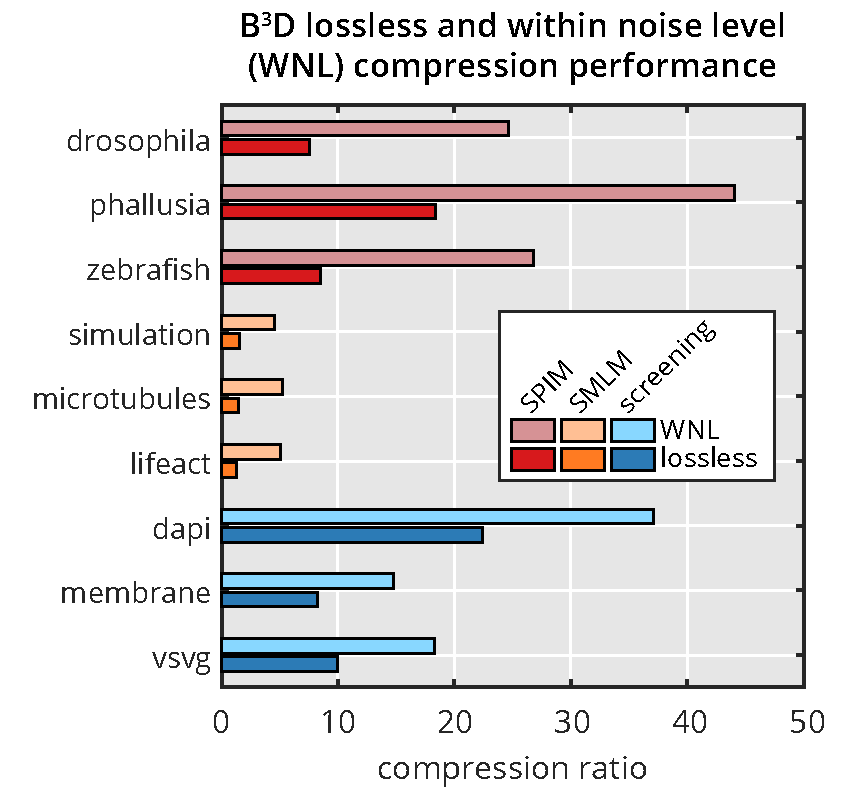
\includegraphics[page=1,height=0.5\textwidth]{Fig1c_compressionBars}
      \bcaption[Within noise level compression performance]{WNL compression performance compared with lossless performance for 9 different dataset representing 3 imaging modalities (SPIM, SMLM, screening). Compression ratio = original size / compressed size. For description of datasets see Table \ref{tab:datasets} in Appendix B.}
      \label{fig:benchmark}
    \end{figure}

    \begin{figure}[tpb]
      \centering
      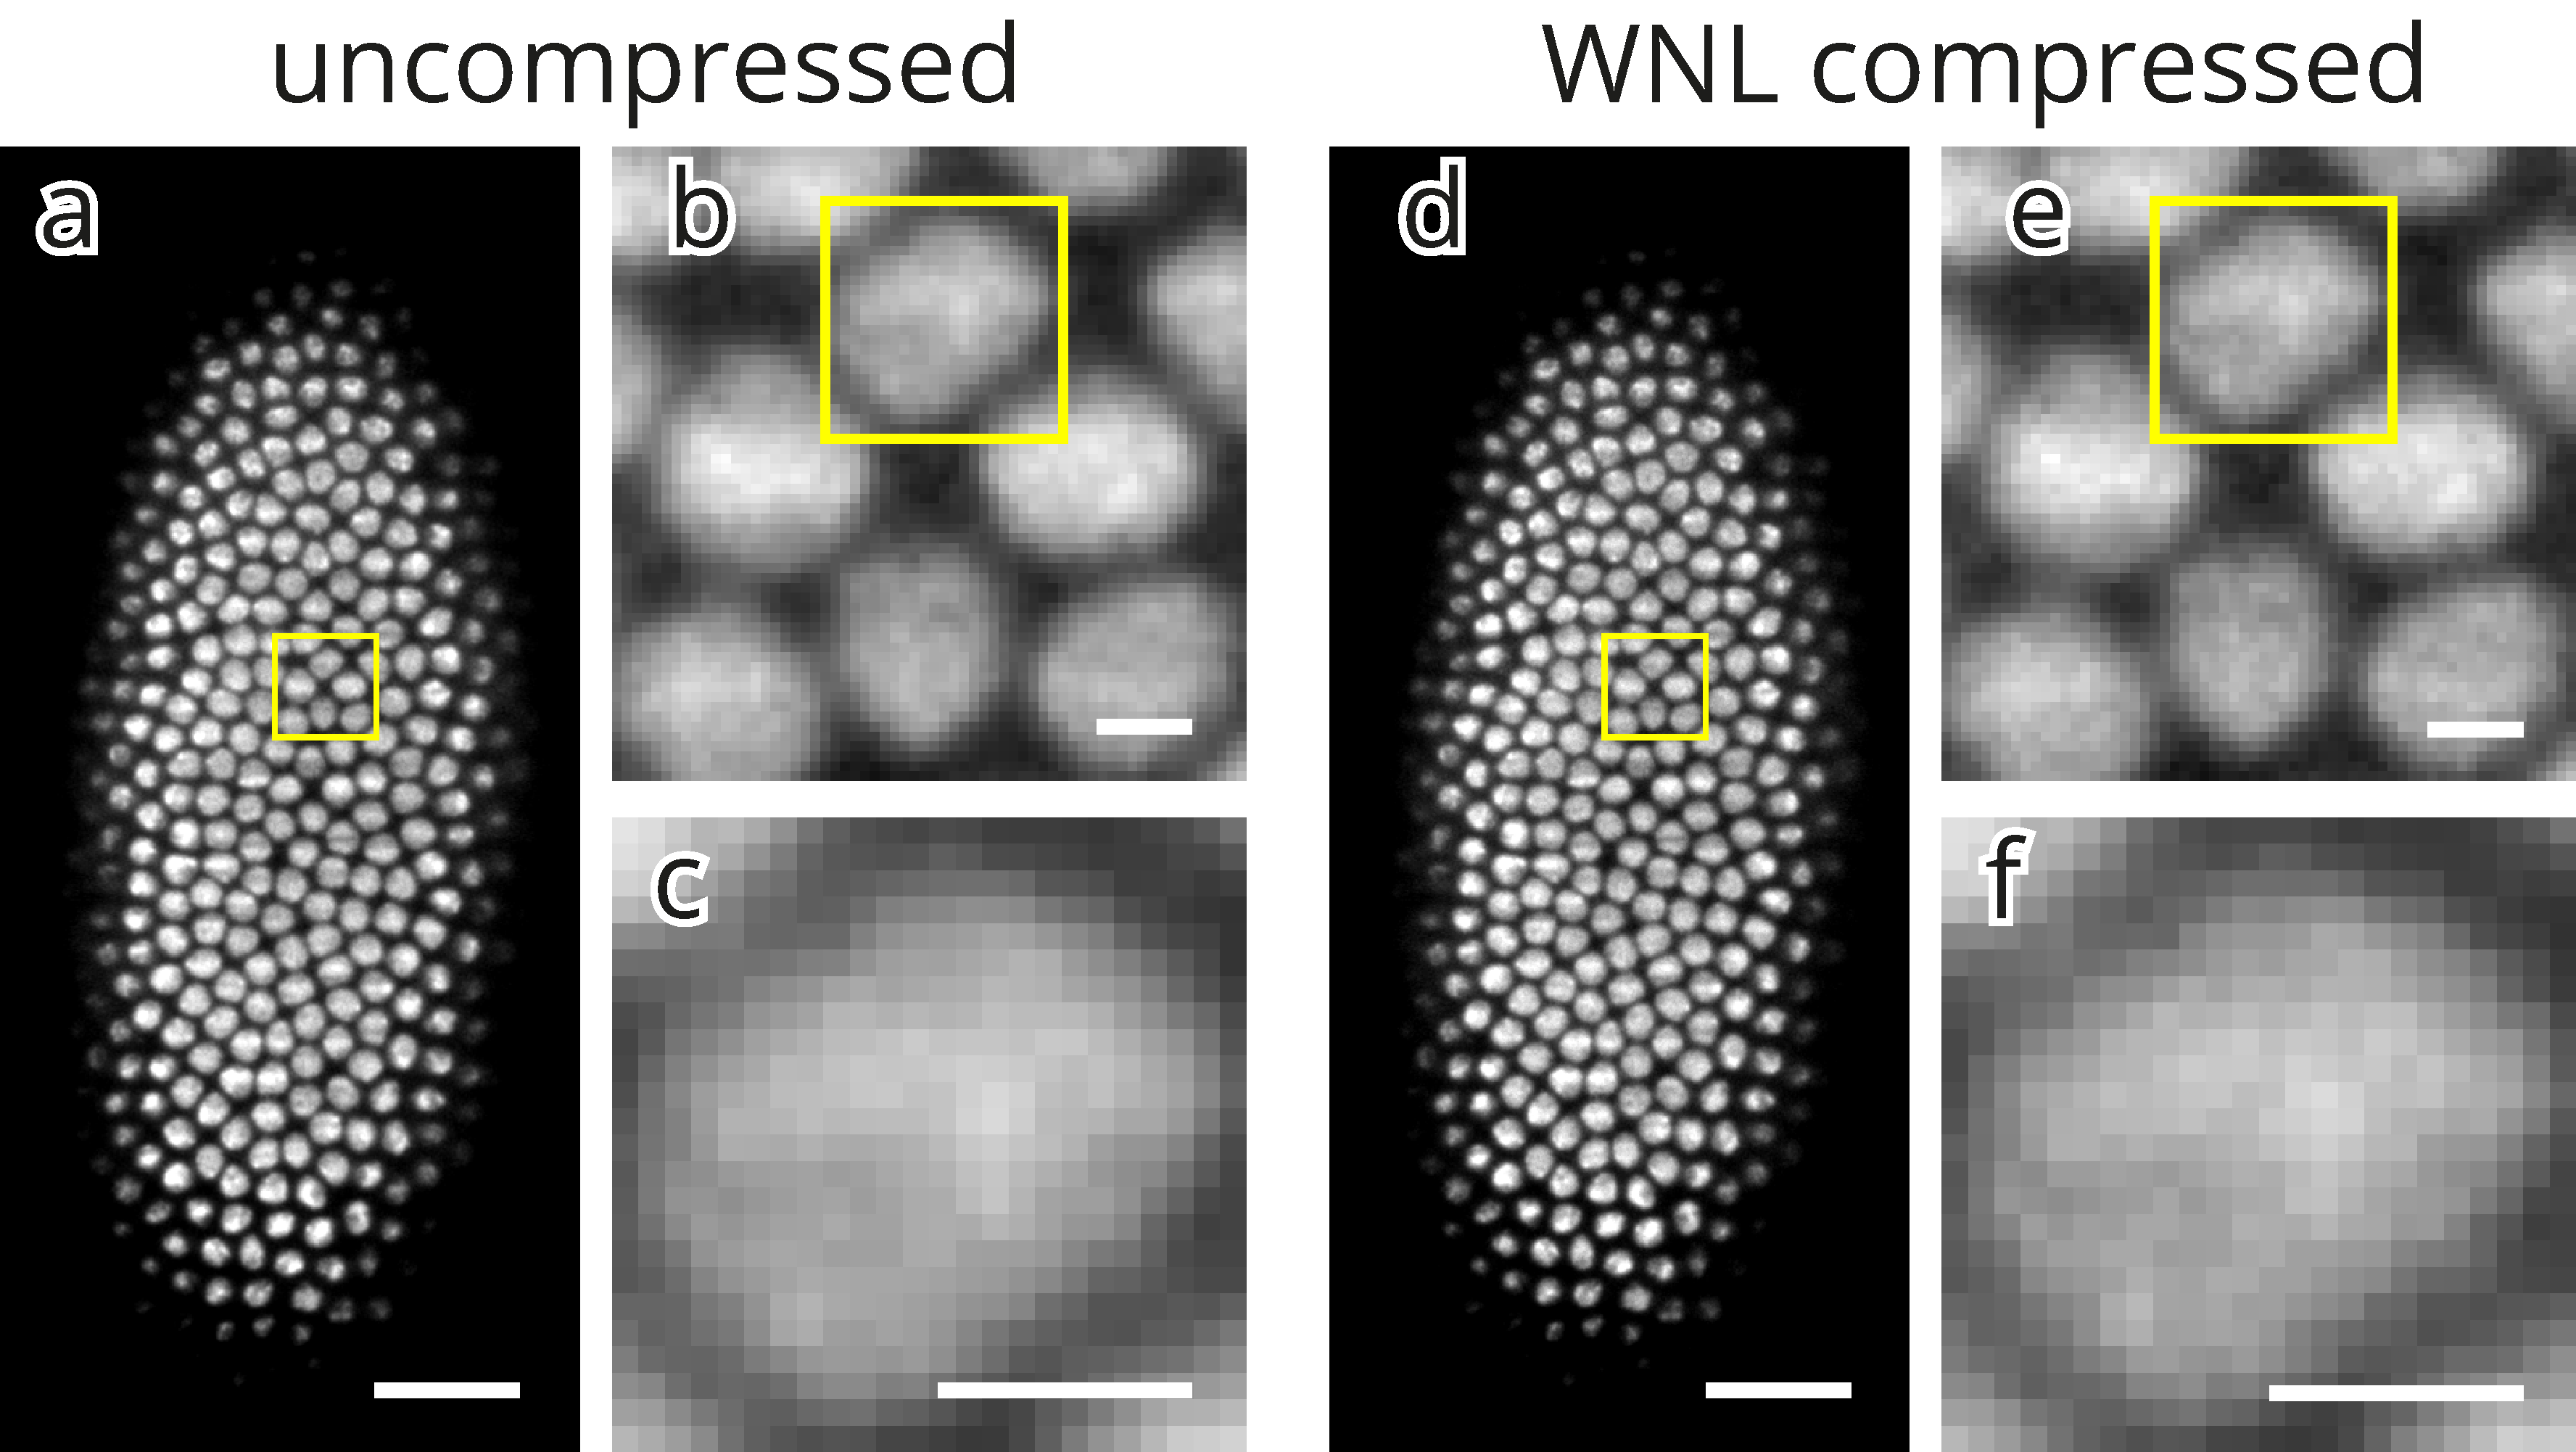
\includegraphics[page=1,width=0.9\textwidth]{wnlSamples}
      \bcaption[Image quality of a WNL compressed dataset]{WNL compression performance compared with lossless performance for 9 different dataset representing 3 imaging modalities (SPIM, SMLM, screening). Compression ratio = original size / compressed size. For description of datasets see Table \ref{tab:datasets}.}
      \label{fig:wnlSamples}
    \end{figure}

    \begin{figure}[tpb]
      \centering
      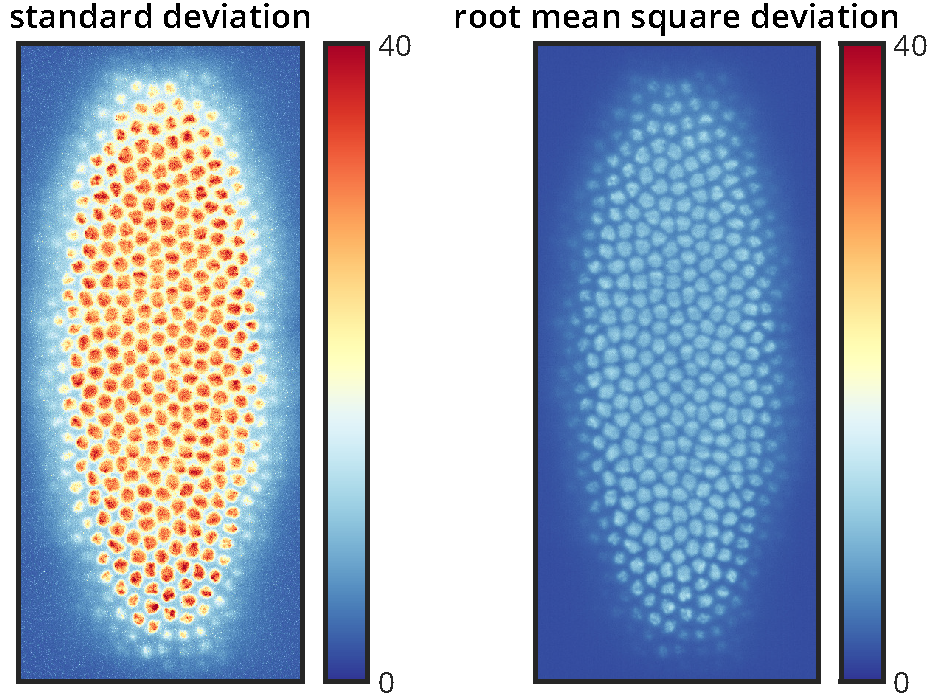
\includegraphics[page=1,width=0.7\textwidth]{SFig4_RMSDvsSD}
      \bcaption[Compression error compared to image noise]{To compare the difference arising from WNL compression to image noise, we imaged a single plane 100 times in a \textit{Drosophila melanogaster} embryo expressing H2Av-mCherry nuclear marker at \SI{38}{ms} intervals. The whole acquisition took \SI{3.8}{s}, for which the sample can be considered stationary. To visualize image noise, the standard deviation was calculated for the uncompressed images (left). All images were then WNL compressed, and the root mean square deviation was calculated compared to the uncompressed images (right). The root mean square deviation on average is 3.18 times smaller than the standard deviation of the uncompressed images.}
      \label{fig:RMSD}
    \end{figure}

    

    \begin{figure}[tpb]
      \centering
      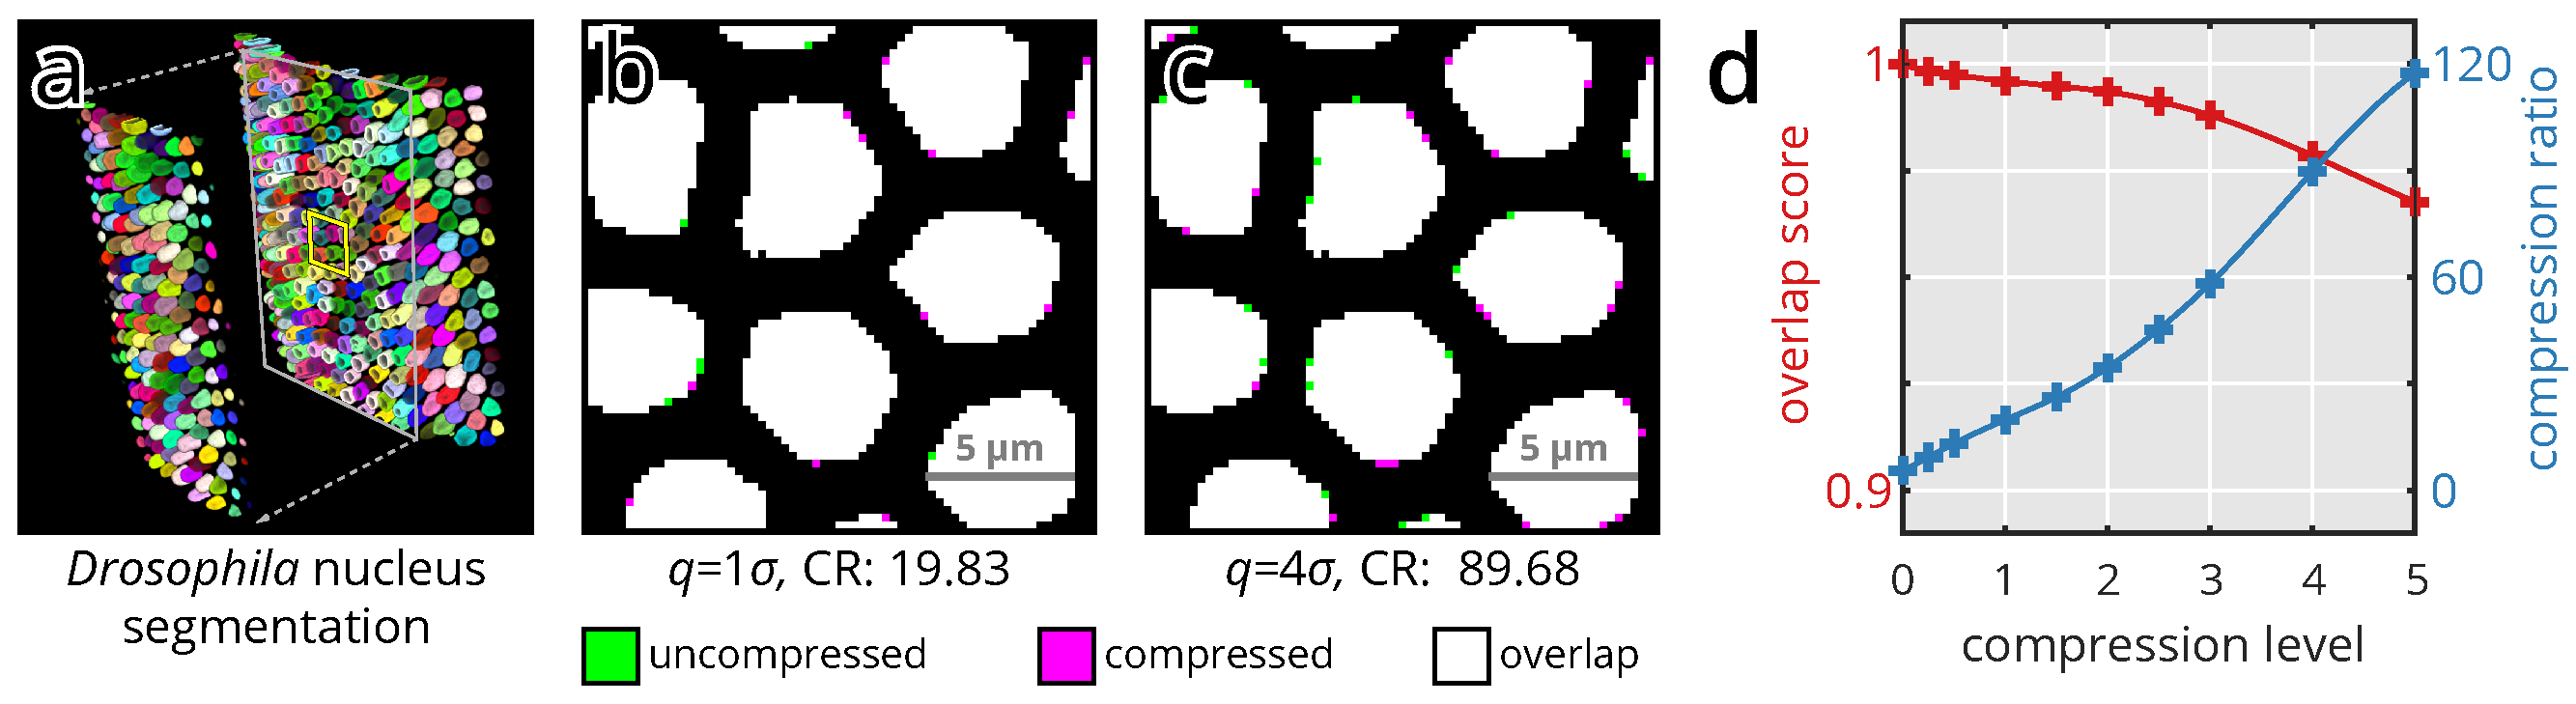
\includegraphics[page=1,width=1\textwidth]{LLvsB3D}
      \bcaption[Influence of noise dependent lossy compression on 3D nucleus segmentation]{A \textit{Drosophila melanogaster} embryo expressing H2Av-mCherry nuclear marker was imaged in MuVi-SPIM \cite{krzic_multiview_2012}, and 3D nucleus segmentation was performed ( "\textbf{Online Methods}") (\textbf{a}). The raw data was subsequently compressed at increasingly higher compression levels, and segmented based on the training of the uncompressed data. To visualize segmentation mismatch, the results of the uncompressed (green) and compressed (magenta) datasets are overlaid in a single image (\textbf{b}, \textbf{c}; overlap in white). Representative compression levels were chosen at two different multiples of the photon shot noise, at q=1$\upsigma$ (\textbf{b}) and q=4$\upsigma$ (\textbf{c}). For all compression levels the segmentation overlap score ( "\textbf{Online Methods}") was calculated and is plotted in (\textbf{g}) along with the achieved compression ratios.}
      \label{fig:wnlDroso}
    \end{figure}

    \begin{figure}[tpb]
      \centering
      \includegraphics[page=3,width=1\textwidth]{LLvsB3D}
      \bcaption[Influence of noise dependent lossy compression on 3D membrane segmentation]{A \textit{Phallusia mammillata} embryo expressing PH-citrine membrane marker was imaged in MuVi-SPIM \cite{krzic_multiview_2012}, and 3D membrane segmentation was performed ( "\textbf{Supplementary Methods}") (\textbf{a}). The raw data was subsequently compressed at increasingly higher compression levels, and segmented using the same settings as the uncompressed data. To visualize segmentation mismatch, the results of the uncompressed (green) and compressed (magenta) datasets are overlaid in a single image (\textbf{b, c}; overlap in white). Representative compression levels were chosen at two different multiples of the photon shot noise, at q=1.6$\upsigma$ (\textbf{b}) and q=4.8$\upsigma$ (\textbf{c}). For all compression levels the segmentation overlap score ( "\textbf{Supplementary Methods}") was calculated and is plotted in (\textbf{d}) along with the achieved compression ratios.}
      \label{fig:wnlPhallusia}
    \end{figure}

    \begin{figure}[tpb]
      \centering
      \includegraphics[page=2,width=1\textwidth]{LLvsB3D}
      \bcaption[Influence of noise dependent lossy compression on single-molecule localization]{Microtubules, immunolabeled with Alexa Fluor 647 were imaged by SMLM (\textbf{a}). The raw data was compressed at increasingly higher compression levels, and localized using the same settings as the uncompressed data. To visualize localization mismatch, the results of the uncompressed (green) and compressed (magenta) datasets are overlaid in a single image (\textbf{b}, \textbf{c}; overlap in white). Two representative compression levels were chosen at q=1$\upsigma$ (\textbf{b}) and q=4$\upsigma$ (\textbf{c}). To assess the effects of compression on localization precision, a simulated dataset with known emitter positions was compressed at various levels. For all compression levels the relative localization error (normalized to the Cramér–Rao lower bound) was calculated and is plotted in (\textbf{d}) along with the achieved compression factors.}
      \label{fig:wnlSMLM}
    \end{figure}

    \begin{figure}[tpb]
      \centering
      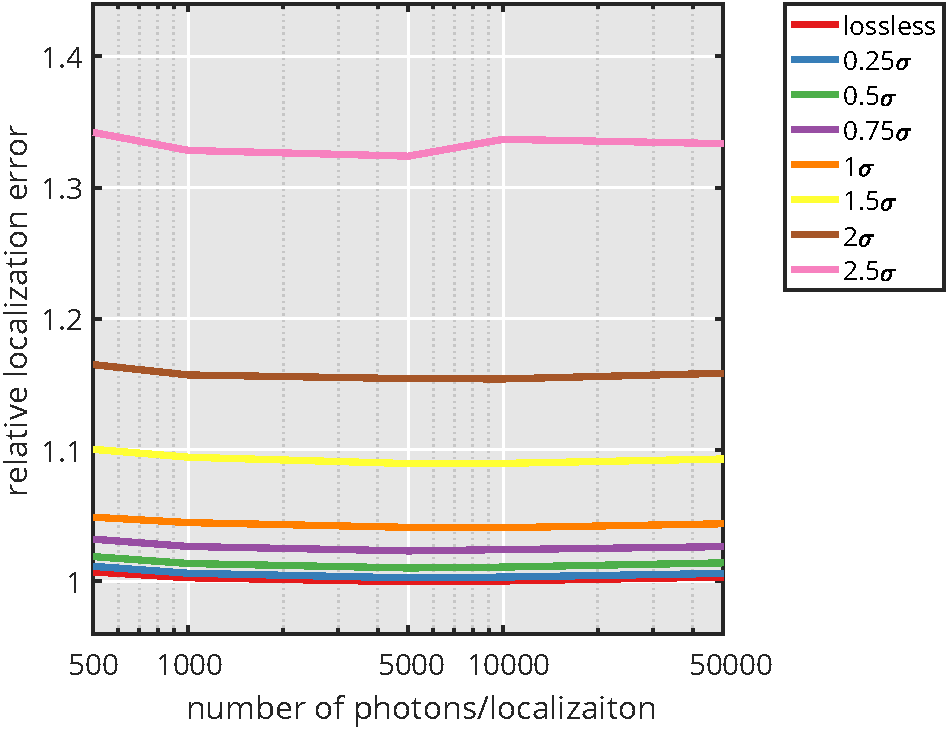
\includegraphics[page=1,width=0.5\textwidth]{SFig6_locprecVsNphotons}
      \bcaption[Change in localization error only depends on selected quantization step]{We simulated multiple datasets ( "\textbf{Supplementary Methods}") with different average photon numbers per localization. Background was kept at a constant average of 20 photons/pixel. Datasets were compressed at multiple compression levels (see legend), and localization error relative to the Cramér-Rao lower bound was calculated. The relative localization error only depends on the compression level, and not on the signal to background illumination ratio.}
      \label{fig:SFig6_locprecVsNphotons}
    \end{figure}

\section{Noise dependent lossy compression}

\section{Methods}
  
\subsubsection{Compression benchmarking}
For all presented benchmarks, TIFF and JPEG2000 performance was measured through MATLAB's imwrite and imread functions, while KLB and \b3d performance was measured in C++. All benchmarks were run on a computer featuring 32 processing cores (2×Intel Xeon E5-2620 v4), \SI{128}{GB} RAM and an NVIDIA GeForce GTX 970 graphics processing unit. Read and write measurements were performed in RAM to minimize I/O overhead, and are an average of 5 runs.

\subsubsection{Light-sheet imaging}
\textit{Drosophila} embryos were imaged in our MuVi-SPIM setup \cite{krzic_multiview_2012} using the electronic confocal slit detection (eCSD) \cite{de_medeiros_confocal_2015}. Embryos were collected on an agar juice plate, and dechorionated in 50\% bleach solution for \SI{1}{min}. The embryos were then mounted in a shortened glass capillary (Brand \SI{100}{\micro l}) filled with 0.8\% GelRite (Sigma-Aldrich), and pushed out of the capillary to be supported only by the gel.

\subsubsection{3D nucleus segmentation}
3D nucleus segmentation of \textit{Drosophila} embryos was performed using Ilastik \cite{sommer_ilastik:_2011}. The original dataset was compressed at different quantization levels, then upscaled in z to obtain isotropic resolution. To identify the nuclei, we used the pixel classification workflow, and trained it on the uncompressed dataset. This training was then used to segment the compressed datasets as well. Segmentation overlap was calculated in Matlab ( "Supplementary Code") using the Sørensen–Dice index \cite{sorensen_method_1948,dice_measures_1945}:
\begin{equation}
  QS = 2 \left| A \cap B \right| / \left( |A| + |B| \right)
\end{equation}
where the sets $A$ and $B$ represent the pixels included in two different segmentations.

\subsubsection{3D membrane segmentation}
Raw MuVi-SPIM recordings of \textit{Phallusia mammillata} embryos expressing PH-citrine membrane marker were kindly provided by Ulla-Maj Fiuza (EMBL, Heidelberg). Each recording consisted of 4 views at 90 degree rotations. The views were fused using an image based registration algorithm followed by a sigmoidal blending of the 4 views. The fused stack was then segmented using the MARS algorithm \cite{fernandez_imaging_2010} with an hmin parameter of 10. The raw data (all 4 views) was compressed at different levels, and segmented using the same pipeline. Segmentation results were then processed in Matlab to calculate the overlap score for the membranes using the Sørensen–Dice index ( "Supplementary Code").

\subsubsection{Single-molecule localization imaging}
In order to visualize microtubules, U2OS cells were treated as in \cite{deschamps_3d_2014} and imaged in a dSTORM buffer \cite{heilemann_subdiffraction-resolution_2008}. In brief, the cells were permeabilized and fixed with glutaraldehyde, washed, then incubated with primary tubulin antibodies and finally stained with Alexa Fluor 647 coupled secondary antibodies. The images were recorded on a home-built microscope previously described \cite{deschamps_3d_2014}, in its 2D single-channel mode.

\subsubsection{Single-molecule localization data analysis}
Analysis of single-molecule localization data was performed on a custom-written MATLAB software as in \cite{deschamps_efficient_2016}. Pixel values were converted to photon counts according to measured offset and calibrated gain of the camera (EMCCD iXon, Andor). The background was estimated with a wavelet filter \cite{izeddin_wavelet_2012}, background-subtracted images were thresholded and local maxima were detected on the same images. 7-pixel ROIs around the detected local maxima were extracted from the raw images and fitted with a GPU based MLE fitter \cite{smith_fast_2010}. Drift correction was performed based on cross-correlation. Finally, images were
reconstructed by filtering out localizations with a high uncertainty (>\SI{30}{nm} and large PSF (>\SI{150}{nm}) and Gaussian rendering.

\subsubsection{Simulation of single-molecule localization data}
Single molecule localization data was simulated in Matlab ( "Supplementary Code") by generating a grid of pixelated Gaussian spots with standard deviation of 1 pixel. With a pixel size of a 100 nm, this corresponds to a FWHM of 235.48 nm. The center of each spot was slightly offset from the pixel grid at 0.1 pixel increments in both x and y directions. To this ground truth image a constant value was added for illumination background, and finally Poisson noise was applied to the image. This process was repeated 10000 times to obtain enough images for adequate accuracy.

\subsubsection{Code availability}
Code used for analyzing data, \b3d source code and compiled binaries, including a filter plugin for HDF5, is available for download at https://git.embl.de/balazs/B3D.
